%
% Unless otherwise indicated, the copyright in this material is 
% owned by Joerg Evermann. This material is licensed to you under the 
% Creative Commons by-attribution non-commercial license (CC BY-NC 4.0)}
%

\section{Introduction}

This chapter provides a brief introduction to legal issues in business analytics. The chapter begins with an introduction to tort law, contracts, licenses, and copyrights, but focuses on data protection and privacy regulation. It concludes with a brief view to AI-specific regulations that are proposed (in Canada) or have already taken effect (in the European Union). 

The chapter takes a Canadian perspective. Canadian tort law is based on common law in the English tradition. As such, some of the concepts and issues discussed in this chapter may be applicable to other common law jurisdictions in the English tradition. On the other hand, the law of the province of Quebec has a different tradition and not all common law concepts apply there. Similarly, the section on copyright law focuses on Canada, although copyright law is internationally relatively harmonized, beginning with the Berne convention of 1886 and through the ongoing activities of the WIPO\footnote{\url{https://www.wipo.int/portal/en/index.html}} \index{WIPO|see{World Intellectual Property Organization}}\index{World Intellectual Property Organization} (World Intellectual Property Organization), such as the WIPO copyright treaty (1996), to which most countries are signatories. The section on information protection and privacy focuses on Canadian federal regulation that applies to commercial activity within Canada. A different set of regulations apply to Canadian federal and provincial governments. Many other jurisdictions around the world also have information protection and/or privacy regulation that may apply to Canadian businesses operating in those jurisdictions, but that may be significantly different from the Canadian regulations. The final two sections discuss Canadian and European Union (EU) legislation around the use of artificial intelligence systems. The Canadian legislation is proposed and, at the time of writing (Sep 2024), is working its way through parliament, while the EU legislation is in force. 

\section{Tort Law}

A tort \index{Tort} is a civil wrong that causes harm to an individual. Tort law governs such civil wrongs or injuries, other than breach of contract, and the remedies for such wrongs and injuries. Torts are typically categorized into torts against the person, property torts, economic torts, dignitary torts, and negligent torts. This section does not provide a comprehensive discussion of tort law but only briefly discusses some torts that may arise in the context of business analytics. 

An important general concept in tort law is that of vicarious liability\index{Vicarious liability}. In particular, employers may be liable for the negligent behaviour, actions, and omissions of their employees. This liability hinges on the definition of an employee versus an independent contract, which has become somewhat blurred in the so-called ''gig economy''. Various tests of employment relationships have been devised and applied by the courts, typically focusing on the exclusivity of the relationship and the level of control exerted by the employer over the employee. 

An example in the context of business analytics may be large scale data collection efforts, for example \href{https://en.wikipedia.org/wiki/Google_Street_View}{Google's Street View} program, may use a fleet of car or bicycle drivers, that may through their actions cause significant harm. Whether the drivers are employees or independent contractors is of importance in assessing the risk. Moreover, the potential harm is not only associated with the risk of traffic accidents, but also potentially other torts such as intentional trespassing or invasion of privacy (intrusion on seclusion). In these cases, the employer may be vicariously liable for the injuries caused by their drivers. 

Damages that can be awarded in tort law are compensatory\index{Damages!Compensatory}, which compensate the injured party financially, and punitive, which are intended to punish the injuring party and deter similar future actions or omissions. The difference is important in that compensatory damages may sometimes be so small as to be considered the normal ''cost of doing business'' by the injuring party. Hence, punitive damages\index{Damages!Punitive} may be awarded that amount to a significant cost to the injuring party in order to form an effective deterrent. Courts may also order an injunction, that is, they prohibit a party from engaging in certain behaviour.

\subsection*{Intentional Torts}

Among the intentional torts, invasion of privacy (intrusion on seclusion) \index{Invasion of privacy}\index{Intrusion on seclusion} may be the most relevant to business analytics endeavours, especially with respect to permissible modes of data collection. Intrusion on seclusion requires intent to intrude, judged subjectively based on the the knowledge of the intruder. The tort also requires the intrusion to be highly offensive, judged objectively from the perspective of a ''reasonable person''. Finally, the tort requires actual harm, e.g. in the form of anguish or emotional suffering. Intrusion on seclusion can be physical, for example, drone-based video collection over private spaces, or virtual, e.g. data scraping off web-sites or illegally accessing databases. Another example is that of employees inappropriately accessing private information held by their own organization (''employee snooping''). However, the standards for offensiveness and actual harm are often difficult to meet, and other privacy laws (cf. Section~\ref{sec:privacy}) may be more applicable in typical cases.

Breach of confidence\index{Breach of confidence} is the tort of disclosing information that is secret, confidential, or private and that was communicated in a situation that implies or imports an expectation of privacy and confidence. The tort requires this information to be of some value or importance and the disclosure to third parties must have caused actual harm. Here too, the standard of actual harm may be difficult to demonstrate and other privacy laws may be more applicable in cases of unauthorized information disclosure. An example in the area of business analytics could be the disclosure of confidential personal information by a data processor to a competitor, with reputational harm to the data owner due to customer complaints, or economic harm to due increased competition.

A related tort that has recently been recognized by the Alberta Court of Queen's Bench and the Saskatchewan Court of King's Bench in 2021 and 2022 respectively. The public disclosure of private facts\index{Public disclosure of private facts} involves publishing an aspect of private life in some form that is highly offensive and is not a legitimate concern to the public. Importantly, both courts determined that the tort is actionable per se, that is, without showing actual damages. As an example in the context of business analytics this tort may arise by publishing a person's medical information with the intent to embarrass or cause reputational damage.

Trespass\index{Trespass to land} to land is the interference with another's right in real property. An example in the business analytics content may occur through video or other sensor data collection. For example, the property rights above land typically extend to some portion of the lower airspace above it. Modern drones commonly use such heights in overflight and may cause ''interference''. However, this tort requires direct and physical interference, a standard that routine data collection behaviour may not rise to. Indirect interference is covered by the tort of nuisance. 

Important defenses against these torts are consent, assumption of risk, or contributory negligence. Both consent and assumption of risk can be expressed or implied. Express assumptions of risk or consent typically take the form of a waiver of liability\index{Assumption of risk}. However, liability waivers must describe specific risks and can absolve a defendant only of liability for negligent, but not reckless conduct. Implied consent is given when a specific harm may be ordinarily or reasonably expected and a person continues to engage in a particular activity. For example, implied consent to data collection may be provided by an online retailer clearly describing the data collection that occurs and a clear statement that continued use of the service implies consent to that data collection. Contributory negligence\index{Negligence!Contributory} is the concept that negligence, i.e. failure to take reasonable care, by the injured party contributed to the injury or harm. This typically leads to some apportionment of loss when both parties contributed to the harm. 

To summarize, the torts described here are intentional torts; an organization or individual must demonstrate intent to harm or injure another party. Additionally, most of these torts are actionable only when harm or injury has actually occurred. 

\subsection*{Negligent Torts and Liability}

Negligence\index{Negligence} is the failure to exercise appropriate care, that is, the breach of the duty of care. A duty of care typically exists where harm or injury is reasonably foreseeable and where there is a required degree of ''proximity'' between the injured party and the defendant. Typical situations in which a duty of care exists are employer-to-employee, manufacturer-to-consumer, provider-to-customer, etc. Throughout the common law countries and jurisdictions, a number of specific tests for the existence of a duty to care have been developed and applied. Negligence requires a breach of the duty to care and a causal proximity to the incurred loss, injury or harm. Causal proximity means that the particular action or omission was the direct or indirect cause of the injury, but at the same time, was not too causally remote or the causal chain interrupted by another event.

An example of negligence in the context of business analytics may be injury caused by decisions or actions from a predictive model if the development or operation of such a decision tool was negligent. For example, the organization failed to examine training data for bias, or failed to appropriately test the finished model. Another example is a data breach by a company that fails to apply security patches or updates to its software, or fails to follow industry security guidelines, and as a result suffers a data loss with consequent injuries or harms to its customers.

Product liability\index{Product liability} is a subset of strict liability in Canadian tort law, which holds manufacturers, distributors, or retailers liable for harm caused by defective or dangerous products, regardless of fault or negligence. With strict liability\index{Strict liability}, the focus is on whether the product was defective or unsafe rather than on the conduct of the defendant and whether the duty of care was breached. In Canadian law, a product is considered defective if there is a design flaw, manufacturing defect, or insufficient warning about its potential risks. In such cases, strict liability allows an injured party to recover damages without needing to prove that the manufacturer was negligent.

In the context of data analytics, strict liability can apply to software products or platforms that handle sensitive data, where defects in the software lead to harm. For example, data analytics software tools should meet high standards for security, reliability, and accuracy. A defective product in this area could lead to data breaches, financial loss, or reputational harm. Consider a retail company that purchases data analytics services from another company to predict customer behaviour. A design flaw in the prediction algorithm means that the retailer consistently misses out on sales as it overprices its products. 

Defences against claims of negligence are assumption of risk and contributory negligence, as discussed above. 

\section{Contracts}

Contracts\index{Contract} are important in many areas of business analytics as they govern the purchase or sale of data, the licensing of data, the collection or creation of data, data processing and data manipulation, the provision of access to or use of analytics services, etc. While the foundations of contract law are important to business analytics, they are not specific or unique to this area. Contract creation in the English law tradition concerns concepts such as offers (willingness to contract with the intent to become binding), invitation to treat (a pre-offer communication), firm offers (valid for a particular time), counteroffers, battle of the form (conflicting terms in offer and acceptance), revocation of offers (prior to acceptance) and acceptance. Contract law introduces the concepts of consideration (the objects or services being exchanged; contracts must involve mutual consideration), privity (being party to a contract; contracts cannot confer rights or obligations on third parties), and assignment (of rights or benefits by one party to another). The law clarifies what form an offer or acceptance must take, how offers, revocations, and acceptance must be communicated, when and whether an offer is deemed to be accepted, etc. For electronic commerce in Canada, the Uniform Electronic Commerce Act (UECA) provides legal recognition of electronic documents, ensures that electronic contracts are enforceable, clarifies electronic communication modalities in contract formation (sending and receiving of electronic documents), and addresses the use of electronic or digital signatures. 

%Contract terms must not include misrepresentations (false or misleading statements). In particular, contract terms may include clauses that exclude or limit liability for a party or make parties waive their rights in case of negligent behaviour of other parties (''liability waivers''). Frequently, contracts also contain indemnification clauses, that is, promises by one party to keep the other from harm.

Specific issues in business analytics sometimes arise in the description of what is being purchased or sold. In particular, data can be sold (that is, the copyright can be assigned to another party), or it can be licensed for use, typically with limitations and restrictions. Data sets may be provided in their entirety as copies, or data may be accessed as needed through electronic means, for example on a subscription basis. In the former case, the contract may specify the rights that are transferred and any limitations on use of the data; in the latter case, the contract may specify the access modalities and rights and obligations of each partner in making available the service and responsible use of the service. Often, data contains personal or protected private information and contracts should contain clauses that specify whether and how such data must be protected. These contract clauses may specify technical or administrative measures, audit and oversight rights, or prescribe employee training and education. 

In business analytics, processing services may be offered and contracted, e.g. for data cleaning, data preprocessing, format shifting, etc. Analytic prediction models may be sold and purchased. For example, trained models are copyrighted and this copyright could be assigned, or a license could be issued, or the model may be accessed to make predictions. For example, when real-time access to a predictive service is purchased in a contract, the buyer should include a liability and indemnification clause that holds the provider liable for wrong or misleading predictions and any injuries suffered because of it. Contracts for accessing services may also specify service levels and performance standards. As an example, a contract may specify the required availability and response time for a real-time prediction service to ensure the service provider maintains appropriate service level. A contract may also impose rate limits for the number of requests per time unit on the part of the service consumer.

In all these cases, the issue of quality, of data or of a service, is important but often difficult to specify in contract terms. For example, how should the quality of a data set be defined so that it can be objectively measured by all parties to the contract? How should thresholds for acceptable quality be set that are unambiguous and understandable by all parties? How should the quality of a trained predictive model be defined? Are there considerations beyond the validation or test error? Who provides the validation or test data to assess the quality? These questions show that considerable effort must be expended on defining appropriate contract clauses. 

\section{Licenses}

A license\index{License} is the permission to use or do something that would otherwise not be permissible. Licenses are transferred as part of a contractual agreement between the rights holder (licensor) and the licensee. A typical use of licenses in business analytics concerns the use of copyrighted material, such as data sets, trained prediction models, or software applications. Licenses can be exclusive, sole, or non-exclusive (ordinary). An exclusive license differs from a sole license in that an exclusive license also prohibits the licensor (rights holder) from engaging in the licensed activity, while a sole license means that only a single license is issued but the rights owner can also engage in the licensed activity. 

Contractual agreements may specify the license to be revocable by the licensor, or to be irrevocable. Licenses may also be time-bound, that is, they have an expiration date, or they can be in perpetuity. Time-boundedness is independent of revocability. For example, a license in perpetuity may be revocable, and an irrevocable license may be bounded in time. 

Licenses may be transferable by the licensee to another party, or non-transferable. Licenses may also provide a (limited) option to sub-license to a third party. When a license is transferred, the original licensee is no longer permitted to engage in the licensed activity, that is, they no longer hold a license, while in the case of sub-licensing, the original licensee retains a license. 

Licenses may grant specific rights or may permit all uses that are normally the right of the author or copyright holder. Licenses may also provide conditions or restrictions for engaging in the licensed activity, and termination of the license when the licensee fails to meet such conditions or violates the restrictions. Finally, licenses may provide or explicitly exclude warranties or provide indemnification clauses.

\section{Copyright}

Copyright\index{Copyright} law governs the rights of authors of an original work, in the sense that the work originated with the author. The scope of what is copyrightable is rather broad, but importantly it does not cover ideas but must involve a ''fixed,'' tangible form. Copyright in Canada includes the rights to reproduce (copy), distribute, publish, and to translate or adapt a work. 

In the context of business analytics, questions may arise with respect to what is copyrightable and whether an activity is reserved for the rights holder. For example, a fact itself is not eligible for copyright protection as it is not an original work, and neither is the simple collection of facts. However, once a collection is curated (that is, some items are removed while others are retained), transformed, or otherwise processed in a manner that involves skill, judgment, or creativity of an individual, the result does constitute an original work eligible for copyright protection. For example, data that is indiscriminately and automatically compiled, e.g. a recording of raw sensor data or the raw text collected by an automated web crawler bot, may not be afforded copyright, but subsequent data cleaning, preprocessing or feature engineering may make the data set eligible for copyright protection.

A particular issue where copyright law may be unclear is the use of data for the training of predictive models. In particular, the question of whether the ingestion of data into model training without making a local copy of that data constitutes reproduction, adaptation, or translation is not yet settled in Canada. Consider text data that is immediately submitted to a tokenizer, converted to integers, and then processed by an embedding layer, all without a copy of the original text being retained. Moreover, the copyright act allows temporary reproductions for technological processes, given that ''the reproduction's only purpose is to facilitate a use that is not an infringement of copyright, and the reproduction exists only for the duration of the technological process'' (Canada Copyright Act, 30.71).

\section{Web Site Data Collection}

Web sites provide a lot of information that is useful for business analytics. Assuming that the data presented on a web site is eligible for copyright protection, the rights holder can limit or prohibit its use by issuing (or withholding) licenses. Typically, web sites provides ''terms of use'' for this purposes. These terms are human-readable documents that specify what rights are given to persons accessing the web site. Terms of use are typically considered valid if clear and reasonable notice is given to them, e.g. by requiring explicit acknowledgment or by providing a conspicuous link to them on a web site. 

However, large-scale web data collection does not rely on human users accessing and reading web sites. Instead, it relies on automated software applications, so called web bots or crawler bots or simply crawlers, that access the content of a web page, process it, and follow any links from one page to another. Crawlers were first devised by the early web search engines, such as Yahoo or Google, to populate their search databases. However, web crawlers are not limited to search engine use. They are now also used, perhaps primarily, to collect data for analytics, e.g. text mining, social network analysis, or collecting image data for the training of predictive models. 

To help control or limit access to the information on a web site by crawlers, web sites can use the Robot Exclusion Protocol\index{Robot exclusion protocol}\index{robots.txt|see{Robot exclusion protocol}}, commonly referred to as the ''robots.txt'' file. Originally devised in 1994 and formally standardized in 2022, a ''robots.txt'' file for a web site specifies in computer-readable format which crawlers or bots are allowed to access which portions of a web site. However, while standardized, not all crawlers obey the limits specified in the robots.txt file and organizations should also consider other measures to prevent unauthorized data scraping, e.g. by configuring their web server to block or ignore such requests or to set access rate limits. 

Figure~\ref{fig:youtuberobots} shows an excerpt of the ''robots.txt'' file of the YouTube web site. The directive \texttt{User-agent:} specifies which type of crawler or bot the following directives in the file apply to. The ''\texttt{Disallow:}'' directive excludes certain portions of the web site. For example, the YouTube ''robots.txt''  file in Figure~\ref{fig:youtuberobots} allows the ''\texttt{Mediapartners-Google*}'' bots access to the entire site, that is, it does not disallow anything for these bots. In contrast, all other bots (''\texttt{User-agent: *}'') are disallowed from certain portions of the site. Contents of the site that are not disallowed are deemed to be allowed. In contrast, the directive ''\texttt{Allow:}'' (not used in the example) works by explicitly permitting access and deeming all not allowed portions to be prohibited. Finally, the ''\texttt{Crawl-delay:}'' (not used by the example) can be used to specify a minimum time (in seconds) before a crawler should access the site again.

In summary, the robot exclusion protocol through the ''robots.txt'' file provides access limits to automated web crawling, but adherence to this protocol by a crawler or bit is voluntary, and not all crawlers understand or honour all directives. Importantly, the directives in this file are not legally binding.

\begin{figure}
\begin{textcode}
# robots.txt file for YouTube
# Created in the distant future (the year 2000) after
# the robotic uprising of the mid 90's which wiped 
# out all humans.

User-agent: Mediapartners-Google*
Disallow:

User-agent: *
Disallow: /api/
Disallow: /comment
Disallow: /feeds/videos.xml

Disallow: /watch_popup
Disallow: /watch_queue_ajax
Disallow: /youtubei/
\end{textcode}
\caption[Example robots.txt file]{Robots.txt file from \url{youtube.com/robots.txt}}
\label{fig:youtuberobots}
\end{figure}

\begin{tcolorbox}[colback=code]
\subsubsection*{Hands-On Exercise}
Identify the robots.txt file of your university web site.
\begin{itemize}
  \item Are there portions of the site a crawler bot is not permitted? Why might this be?
  \item Are there different directives for different crawlers?
  \item Are there limits on crawl frequency?
\end{itemize}
\end{tcolorbox}

\section{Information Protection and Privacy Legislation\\ in Canada}
\label{sec:privacy}

This section presents an overview over the information protection and privacy legislation in Canada. The section focuses on the Personal Information Protection and Electronic Documents Act (PIPEDA).

\begin{tcolorbox}[colback=alert]
\subsubsection*{Resources}
Information in this section is based on and adapted from that provided by the Office of the Privacy Commissioner of Canada on the \href{https://www.priv.gc.ca/en/privacy-topics/privacy-laws-in-canada/the-personal-information-protection-and-electronic-documents-act-pipeda/p_principle/}{PIPEDA web page} and related pages. In particular, the following web pages are useful introductory resources:
\begin{itemize}
   \item \href{https://www.priv.gc.ca/en/privacy-topics/privacy-laws-in-canada/the-personal-information-protection-and-electronic-documents-act-pipeda/pipeda-compliance-help/02_05_d_55_tips/}{10 Tips for avoiding complaints} is a short list of recommendations for businesses. 
   \item \href{https://www.priv.gc.ca/media/2038/guide_org_e.pdf}{Privacy Guide for Businesses} is a concise guide to responsibilities under PIPEDA.
   \item \href{https://www.priv.gc.ca/en/privacy-topics/privacy-laws-in-canada/the-personal-information-protection-and-electronic-documents-act-pipeda/pipeda-compliance-help/pipeda-interpretation-bulletins/}{PIPEDA Interpretation Bulletins} provide commentary based on legal precedents and interpretations by courts of the PIPEDA legislation.
   \item \href{https://www.priv.gc.ca/en/privacy-topics/privacy-laws-in-canada/the-personal-information-protection-and-electronic-documents-act-pipeda/pipeda-compliance-help/issue-specific-guidance-for-businesses/}{Issue specific guidance for businesses} provides guidance on a number of specific issues, ranging from e-marketing to manufacturing internet-of-things devices.
   \item \href{https://www.priv.gc.ca/en/privacy-topics/privacy-laws-in-canada/the-personal-information-protection-and-electronic-documents-act-pipeda/pipeda-compliance-help/pipeda-compliance-and-training-tools/gl_acc_201204/}{Getting accountability right} provides a guide for businesses to design and implement an ''accountable organization''. 
\end{itemize}
\end{tcolorbox}

PIPEDA\index{Personal Information Protection and Electronic Documents Act}\index{PIPEDA!see{Personal Information Protection and Electronic Documents Act}} is a federal legislation that applies to commercial activity in all Canadian provinces, unless the activity takes place solely within a province has passed substantially similar provincial legislation. At the time of writing (Sep 2024), this is only applies to British Columbia and Ontario. Importantly, PIPEDA does not apply to the Canadian federal government or the provincial governments. Information protection for the former is subject to the Privacy Act and the Access to Information Act, while information protection for provincial governments is regulated by specific provincial acts, for example, the Access to Information and Protection of Privacy Act (ATIPPA) in Newfoundland and Labrador.

PIPEDA establishes the Office of the Privacy Commissioner of Canada (OPC) that is responsible for overseeing compliance with both the Privacy Act and PIPEDA. In particular, the OPC has the power to investigate complaints about compliance, but has no enforcement power. Upon investigation of a complaint, the OPC issues a report that makes non-binding recommendations. This report also provides leave for the complainant to take their case to federal court. 

\subsection*{Personal Information}

Personal information\index{Personal information} in PIPEDA means information about an identifiable individual. This definition is very broad and covers a range of data. However, specifically exempt is contact information that an organization uses solely for communication with employees. Examples of personal information are:

\begin{itemize}
   \item Name, age, weight, height
   \item Address and communication info, for example email addresses and phone numbers.
   \item Medical information, such as medical records, clinical notes, and prescriptions for medication.
   \item Financial information, for example income, purchases, financial transactions, debt and credit information.
   \item Race and ethnicity, marital status and religion.
   \item Biometrics, such as DNA, voice-prints, and fingerprints.
   \item Location information, for example GPS or RFID based location information (if linked to an individual), an IP address (if linked to an individual).
   \item Education information, such as transcripts, grades, scholarship applications, scholarships.
   \item Employment information, such as employment records, performance evaluations and appraisals, salary and benefits information.
   \item Opinions held and comments expressed by an individual.
\end{itemize} 

Importantly, anonymous information is also considered personal if there is a serious possibility that an individual could be identified, based on that information alone or in combination with other information. This interpretation presents a serious challenge for anonymizing information when large data sets with multiple variables are stored.

\subsection*{Fair Information Principles}

PIPEDA is structured around ten ''Fair Information Principles'' that govern the collection, use, disclosure, and retention of personal information, as well as the rights of individuals with respect to the organizations holding that data. 

\begin{enumerate}
   \item Be accountable
   \item Identify the purpose
   \item Obtain valid, informed consent
   \item Limit collection
   \item Limit use, disclosure and retention
   \item Be accurate
   \item Use appropriate safeguards
   \item Be open
   \item Give individuals access
   \item Challenging compliance
\end{enumerate}

Additionally, PIPEDA provides for mandatory breach reporting by organizations, a process for individuals to complain about compliance to the OPC, and the authority of the OPC to audit organizations for PIPEDA compliance. The remainder of this section will examine each fair information principle in more detail.

\subsection*{PIPEDA Fair Information Principle 1: Accountability}

The accountability\index{Accountability} principle is an overarching principle that requires organizations to be compliant with PIPEDA and all ten fair information principles\footnote{\href{https://www.priv.gc.ca/en/privacy-topics/privacy-laws-in-canada/the-personal-information-protection-and-electronic-documents-act-pipeda/p_principle/principles/p_accountability/}{PIPEDA Fair Information Principle 1 -- Accountability (OPC)}}. Specifically, organizations are required to appoint a person responsible and accountable for compliance with PIPEDA. This person or office is responsible for protecting personal information, including any information that is transferred to third parties and agents, e.g. for processing or for other purposes. In larger companies, this may take the form of a dedicated privacy officer, possibly with an office and staff. This person or office must have the support of the senior management, must be appropriately resourced, and must have the authority to take action on privacy issues. The reporting lines, both from this person, e.g. to the CEO or board of directors, but also to this person, e.g. from other employees or managers of the organization, should be explicitly defined. 

The OPC recommends that organizations develop and implement a comprehensive privacy management program to demonstrate accountability\footnote{\href{https://www.priv.gc.ca/en/privacy-topics/privacy-laws-in-canada/the-personal-information-protection-and-electronic-documents-act-pipeda/pipeda-compliance-help/pipeda-compliance-and-training-tools/gl_acc_201204/}{Getting accountability right with a privacy management program (OPC)}}. A key element of such a program is an information inventory that identifies all personal information held or controlled by the organization, including its sensitivity, when and why it was collected, when and how consent for the collection was obtained, how and where it is stored, who uses or accesses it, and who it is shared with or disclosed to.

A second element is a set of policies that govern how an organization engages in the collection, use and disclosure of personal information, organizational rules on gaining consent and notifying individuals about their information. A policy should also define how individuals can exercise their rights under PIPEDA to access and correct their information. The policy might specify how the organization determines the identity of the requesting individual, how it identifies and locates the requested information, how it redacts information about other individuals, and how it deals with correction requests. A policy should define the retention and disposal of information, for example, how long information is retained, and when the retention period may be extended. Disposal is more than the deletion of a data file and policies should specify disposal mechanisms for different types of information and different media. An information security policy specifies administrative, physical, and technological security controls, such as physical access to the computer room, encryption of data at rest and in transit, required or acceptable authentication and authorization mechanism, and role-based access privileges to the data. Individuals have the right under PIPEDA to challenge organizations to demonstrate compliance. Policies should be in place how such challenges are managed and processed.

A third element of a privacy management program is a set of risk and threat assessments tools and mechanisms for all business operations. New initiatives, new products, or new business processes should routinely undergo a risk or threat assessment with respect to personal information protection and privacy in the normal course of their development. This includes information system development, business process redesigns, product design, outsourcing agreements, new venture creation, new market development, etc. 

Employee training and education are another element of a comprehensive privacy management program. These should foster an organizational culture of privacy awareness and also convey knowledge about the specific policies and procedures. One important way in which PIPEDA may be violated is by ''employee snooping'', that is, unauthorized access by employees to and use or disclosure of such information for purposes for which it was not collected. Training should be provided when employees first enter an organization as well as on a recurring schedule, and in particular when the organization makes significant changes to its policies or procedures. 

Because PIPEDA requires organizations to report privacy breaches to the OPC in certain situations, breach and incident management procedures must be in place that govern who reports a breach, when a breach is reported, when and how affected individuals are notified, etc. 

An important element of a privacy management program is the management of external service providers, agents, or other third parties that data is shared with or disclosed to. While transfer of data for processing constitutes use of data, rather than disclosure, the organization owning the data remains accountable for its protection and privacy. Therefore, data transfer for processing requires contractual agreements to be in place that provide an equivalent protection of information at third parties. This ranges from specifying permitted uses to required technological security measures, and may include required employee training and specific administrative responsibilities. Such contracts must be managed and third party compliance with such contracts should be ensured by regular audits. Of particular importance in trans-border data sharing arrangements are the legal protections of information\footnote{\href{https://www.priv.gc.ca/en/privacy-topics/airports-and-borders/gl_dab_090127/}{Guidelines for processing personal data across borders (OPC)}}. Foreign governments may have rights to access information that make it difficult to comply with PIPEDA, for example through financial disclosure regulations, or access to information for police and national security purposes.

Finally, a privacy management program should have procedures for handling external communication that specify how policies are communicated, how individuals can contact the organization, when and how individuals are notified of transfer or disclosure of their information, etc.

With these elements in place, accountable privacy management requires periodic assessment of the effectiveness of these elements and controls and document compliance by the organization with their policies through audits and documentation of audit findings. Important in this context is the authority of the OPC to audit organizations for PIPEDA compliance. This means that, for example, it is insufficient to offer training to employees; training participation and outcomes must be evaluated and recorded to demonstrate effectiveness. Similarly, it is insufficient to merely put in place an information access policy; access to information should be monitored and relevant documentation should be retained to demonstrate compliance. 

Policies and procedures should be periodically assessed as to whether they reflect the latest OPC guidelines and industry best practices. As noted above, the OPC may make recommendations as the result of a complaint, and individuals may bring cases to federal court. Both mechanisms should lead organizations to adopt any resulting best practices or requirements. 

\subsection*{PIPEDA Fair Information Principle 2: Identifying Purpose}

PIPEDA requires organizations to identify and document the purpose for which information is collected\footnote{\href{https://www.priv.gc.ca/en/privacy-topics/privacy-laws-in-canada/the-personal-information-protection-and-electronic-documents-act-pipeda/p_principle/principles/p_purposes/}{PIPEDA Fair Information Principle 2 -- Identifying purposes (OPC)}}. The purpose for collection must be communicated to individuals when requesting consent for collection. The purpose for collection must be specific and considered appropriate by a ''reasonable person'', that is, not overly broad and must be related to the business activities of the organization. Importantly, when information that is already collected is to be used for a different purpose, renewed consent must be obtained. 

\subsection*{PIPEDA Fair Information Principle 3: Obtaining Consent}

Obtaining consent for collection, use, and disclosure of information is the aspect of PIPEDA that has drawn the most attention by consumers, the OPC, and the courts. Consent\index{Consent} must be meaningful and valid\footnote{\href{https://www.priv.gc.ca/en/privacy-topics/privacy-laws-in-canada/the-personal-information-protection-and-electronic-documents-act-pipeda/p_principle/principles/p_consent/}{PIPEDA Fair Information Principle 3 -- Consent (OPC)}}. This requires that individuals understand what they are consenting to, that is, what information is collected, for what purpose, who it is shared with or disclosed to, and what are the potential risks or harms that arise from the collection, use, and disclosure. Since PIPEDA came into force, the requirements for meaningful and valid consent have been clarified by the OPC and the courts\footnote{\href{https://www.priv.gc.ca/en/privacy-topics/collecting-personal-information/consent/gd_53_201805/}{Guidance on inappropriate data practices: Interpretation and application of subsection 5(3) (OPC)}}. In particular, the information about collection, use, and disclosure of information must be clearly and explicitly communicated in understandable form. Individuals must be presented with a clear choice to provide or withhold consent, and the consent process must be user-friendly. Organizations are required to provide a way for individuals to withdraw or revoke their consent, and must act as soon as feasible on such a revocation or withdrawal. Organizations must also re-obtain consent if information is to be used for a different purpose, or if the organization makes significant changes to its privacy practices, e.g. sharing information with different third parties, or with third parties located in different jurisdictions, etc. Finally, organizations are required to retain appropriate records to demonstrate compliance with the PIPEDA consent requirement. 

Importantly, the OPC and the court has held that consent is necessary but not sufficient for data collection. In combination with principle 2 (identifying purpose), the information collection must also serve a real and genuine business interest, and the loss of privacy must be proportional to the benefits gained by individual. 

The OPC considers certain types of data collection to be ''no-go zones'', that is, they are considered inappropriate even with consent\footnote{\href{https://www.priv.gc.ca/en/privacy-topics/collecting-personal-information/consent/gd_53_201805/}{Guidance on inappropriate data practices: Interpretation and application of subsection 5(3) (OPC)}}:
\begin{itemize}
   \item Collection, use, or disclosure that would be illegal
   \item Profiling or categorization that leads to unfair, unethical, or discriminatory treatment
   \item Collection, use, or disclosure that is likely to cause significant harm
   \item Publishing information with intent to charge for removal
   \item Requiring social media passwords for employee screening
   \item Surveillance through an individual's own devices
\end{itemize}

Consent may be provided explicitly or implicitly but the collection, use, and disclosure of sensitive information requires explicit consent. Health or medical information and financial information is considered sensitive, but the sensitivity of information also depends on the purpose for which it is collected and the context in which it is used. The following examples are based on OPC recommendations and court decisions\footnote{\href{https://www.priv.gc.ca/en/privacy-topics/privacy-laws-in-canada/the-personal-information-protection-and-electronic-documents-act-pipeda/pipeda-compliance-help/pipeda-interpretation-bulletins/interpretations_07_consent/}{Interpretation Bulletin: Form of Consent (OPC)}}:

\begin{itemize}
   \item The number of weekly gym visits may not require explicit consent, but disclosure to work team members may make this information sensible, therefore requiring explicit consent.
   \item The viewing of health-related websites is sensitive information.
   \item While an email address is not normally considered sensitive information, it may be sensitive when it indicates a social connection between individuals.
   \item Palm-vein scanning in the context of authentication to a computer system or for physical access control is not sensitive if the scan is not stored and is immediately transformed.
   \item Disclosure of sensitive financial information requires explicit consent, while disclosure only of customer contact information for financial marketing is not considered sensitive and may only require opt-out consent.
   \item Purchasing habits and transaction records are sensitive information, whose collection, use, and disclosure requires explicit consent.
   \item Voice prints collected for purposes of authentication to a computer system are not considered sensitive information.
   \item Non-users of social networking sites would not reasonably expect the use of their email addresses for creating links. Hence, this use requires explicit consent.
   \item In initiating a complaint procedure, medical information may be be disclosed to the defendant in order to defend themselves through implied consent.
   \item GPS location data may be collected by implied consent for the purposes of improving productivity, or protecting and managing company assets, but not for employee evaluation.
\end{itemize}

Organizations may collect information by offering opt-out consent whereby consent is assumed until and unless an individuals withdraws that consent. Opt-out consent is acceptable only under specific conditions\footnote{\href{https://www.priv.gc.ca/en/privacy-topics/privacy-laws-in-canada/the-personal-information-protection-and-electronic-documents-act-pipeda/pipeda-compliance-help/pipeda-interpretation-bulletins/interpretations_07_consent/}{Interpretation Bulletin: Form of Consent (OPC)}}:

\begin{itemize}
   \item The information is non-sensitive in nature and in context, and
   \item Sharing of information is limited and well-defined, and
   \item The organization's purposes are limited and well-defined and clearly stated at time of collection, and
   \item An opportunity for opt-out is offered as soon as possible, and
   \item The procedure for opting out must be convenient, and
   \item The opt-out takes effect immediately, and
   \item The opt-out must be communicated to related businesses, subsidiaries, or third parties that use the collected data.
\end{itemize}

\begin{tcolorbox}[colback=code]
\subsubsection*{Hands-On Exercise}
Consider your bank or communications provider or other large organization you regularly deal with. 
\begin{itemize}
  \item What information have they collected and for what purpose?
  \item How have you provided meaningful consent? Did you have a clear choice?
  \item What is process for withdrawing or revoking consent?
\end{itemize}
\end{tcolorbox}

\subsection*{PIPEDA Fair Information Principle 4: Limiting Collection}

As noted above, the information collected about individuals must fulfill a legitimate and identified purpose\footnote{\href{https://www.priv.gc.ca/en/privacy-topics/privacy-laws-in-canada/the-personal-information-protection-and-electronic-documents-act-pipeda/p_principle/principles/p_collection/}{PIPEDA Fair Information Principle 4 -- Limiting Collection (OPC)}} and it must be fair and lawful. Organizations should identify the information they collect in information management policies. In general, limiting the amount of collected information also reduces the risk to an organization from accidental disclosure or inappropriate use. 

Video data collection may play an important role in the context of business analytics, whether it is for automatic event detection or to serve as training data for prediction models. The OPC provides a number of guidelines\footnote{\href{https://www.priv.gc.ca/en/privacy-topics/surveillance/video-surveillance-by-businesses/gl_vs_080306/}{Guidelines for Overt Video Surveillance in the Private Sector (OPC)}} for PIPEDA compliant video data collection. 

\begin{itemize}
   \item Organizations should evaluate whether less privacy-intensive alternatives can achieve the same purpose. For example, organizations may consider infrared cameras, LIDAR or radar sensors to record the movement of individuals, but these do not normally allow identifying individuals.
   \item Organizations must establish a clear business purpose and use video data collection only for that purpose.
   \item Organizations should develop a policy for the use of video data that limits how and when such data can be accessed, viewed, and processed.
   \item Organizations should limit the viewing angle and viewing range of cameras as far as possible and not not record audio unless necessary. In particular, video data collection is not permissible in areas where individuals have heightened expectations of privacy.
   \item Organizations must inform the public that surveillance is taking place using clear and understandable notices before individuals enter an area that is under video surveillance.
   \item The collected video data must be stored securely and destroyed when it is no longer required for the purpose for which it was collected.
   \item Organizations must allow individuals access to their video data. At the same time, individuals must not be able to view information about others. This may require organizations to technologically blur or otherwise make unrecognizable third parties in video data.
   \item While video data is often collected and processed automatically and without human involvement, organizations should train and educate any human camera operators and third party data processors on privacy obligations. 
   \item Organizations should periodically evaluate the need for continued video surveillance.
\end{itemize}

\subsection*{PIPEDA Fair Information Principle 5: Limiting Use, Disclosure, and Retention}

Organizations must limit the use, disclosure, and retention of data to identified purposes for which it has obtained consent from the individual\footnote{\href{https://www.priv.gc.ca/en/privacy-topics/privacy-laws-in-canada/the-personal-information-protection-and-electronic-documents-act-pipeda/p_principle/principles/p_use/}{PIPEDA Fair Information Principle 5 -- Limiting use, Disclosure, and Retention (OPC)}}. Renewed consent is required when the data is to be used for a new purpose or is disclosed to a different set of third parties. Organizations should also identify the normal retention period for data and the circumstances that require an extension of the retention period. For example, financial regulations may specify minimum retention periods; when an individual has filed a complaint, information must be retained until resolution of the complaint. Organizations must also restrict access to only those employees that require access to fulfill the purpose for which the information is to be used. Organizations should have in place administrative, technological, and physical measures to authenticate and authorize individuals to access personal information.

Disposal of information should be governed by a policy and follow a process that is appropriate to the sensitivity of the information and to the medium on which it is stored. Disposal must include any back-ups and copies of the information, including those at third party service providers and other parties to which it has been disclosed. Contractual agreements should be in place to govern information disposal by third parties and contractual compliance should be regularly audited. Importantly, information to be disposed of must be maintained securely until disposal is complete and verified. 

\begin{figure}[b]
\centering
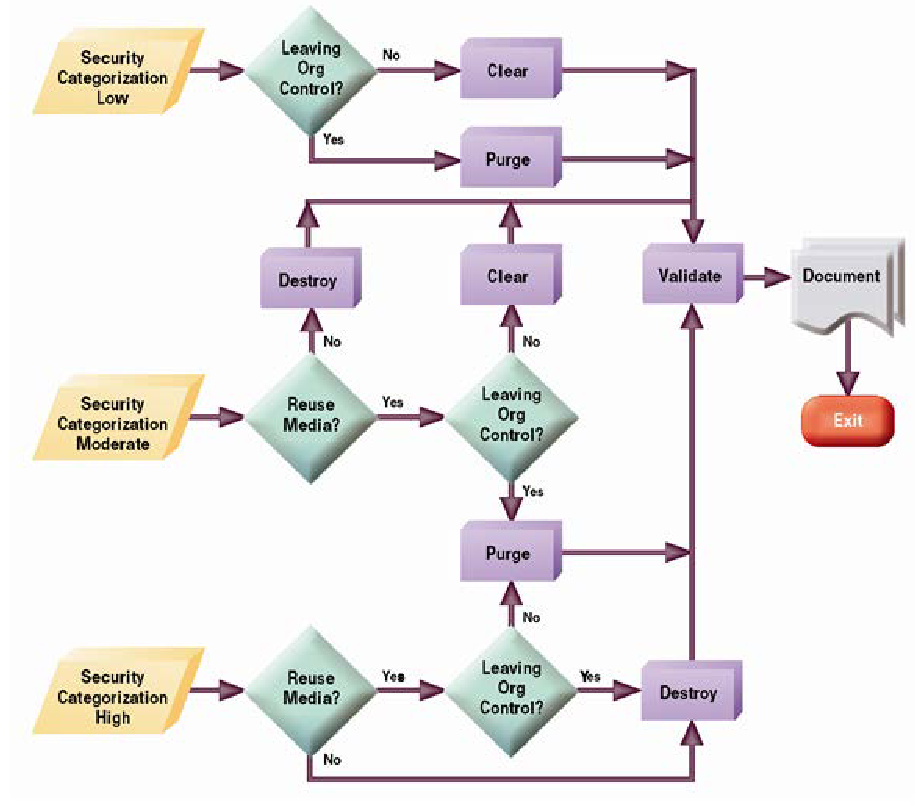
\includegraphics[width=.75\textwidth]{screen1.png} \\ 

\vspace{\baselineskip}

\tiny \textbf{Source:} \href{https://nvlpubs.nist.gov/nistpubs/SpecialPublications/NIST.SP.800-88r1.pdf}{NIST SP 800-88R1 --- Guidelines for Media Sanitization, National Institute of Standards and Technology, US}
\caption{US NIST guidelines for media sanitization}
\label{fig:nist}
\end{figure}

Figure~\ref{fig:nist} shows guidelines for media sanitization by the United States National Institute for Standards and Technology (NIST). Depending on the sensitivity of the information and whether the medium leaves organizational control, three different types of disposal are used. ''Clearing'' information is the simple deletion of information. However, on most computer systems this means that the information remains on the storage medium, e.g. the hard drive, but the space is marked as available for overwriting with new data. In other words, the information can easily be recovered. ''Purging'' of information explicitly overwrites deleted information with zeros or random information or exposes magnetic storage media to strong magnets, so that the deleted information cannot normally be recovered. However, forensic laboratories with the right equipment may even in these circumstances be able to recover at least some of the information. ''Destroying'' storage media means physical destruction so that even forensic recovery techniques are unable to restore the information. This typically involves finely shredding hard drives or vaporizing them using extremely high temperatures. Important in the process shown in Figure~\ref{fig:nist} is the need to validate and document the disposal of information in all cases. 

\subsection*{PIPEDA Fair Information Principle 6: Ensure Accuracy}

PIPEDA requires organizations to ensure the accuracy, completeness and currency of information about individuals\footnote{\href{https://www.priv.gc.ca/en/privacy-topics/privacy-laws-in-canada/the-personal-information-protection-and-electronic-documents-act-pipeda/p_principle/principles/p_accuracy/}{PIPEDA Fair Information Principle 6 -- Accuracy (OPC)}}. This means that collection dates for all information should be recorded and information should be updated if necessary. Organizations should define policies and procedures for ensuring accuracy, e.g. by regularly verifying information with the individual about which it is held, and communicate and follow those procedures. 

Over the years, the OPC and courts have interpreted and clarified this principle\footnote{\href{https://www.priv.gc.ca/en/privacy-topics/privacy-laws-in-canada/the-personal-information-protection-and-electronic-documents-act-pipeda/pipeda-compliance-help/pipeda-interpretation-bulletins/interpretations_04_accuracy/}{Interpretation Bulletin: Accuracy (OPC)}}:
\begin{itemize}
\item Information need only be as accurate as is necessary for the purpose for which the information is collected. 
\item Industry standards for data accuracy are not always an appropriate reference, as these standards may be too low to satisfy the PIPEDA requirements. 
\item The responsibility for ensuring information accuracy rests with the organization that holds the data, not the individual. That is, the organization must be pro-active in verifying the data it holds. \item Any updates to data must also be communicated in a timely manner to any third parties that hold copies of the data for processing. 
\end{itemize}

\subsection*{PIPEDA Fair Information Principle 7: Information Safeguards}

Organizations need to safeguard the information they collect through measures that are commensurate with and appropriate for the sensitivity of the information \footnote{\href{https://www.priv.gc.ca/en/privacy-topics/privacy-laws-in-canada/the-personal-information-protection-and-electronic-documents-act-pipeda/p_principle/principles/p_safeguards/}{PIPEDA Fair Information Principle 7 -- Safeguards (OPC)}}. Such measures can be administrative, technological, or physical in nature. PIPEDA does not specify particular safeguard mechanisms. Instead, organizations must continually ensure they adequately protect the information and evolve their safeguards as technology evolves. An example of administrative safeguards are role-based access permission and employee training. Encryption and password-based access restrictions are examples of technological safeguards. 

Since PIPEDA was enacted, the interpretation of the requirement to safeguard information has evolved and been interpreted in light of complaints\footnote{\href{https://www.priv.gc.ca/en/privacy-topics/privacy-laws-in-canada/the-personal-information-protection-and-electronic-documents-act-pipeda/pipeda-compliance-help/pipeda-interpretation-bulletins/interpretations_08_sg/}{Interpretation Bulletin: Safeguards (OPC)}} brought before the OPC:
\begin{itemize}
  \item Safeguards must be commensurate with the sensitivity of information. For example, highly sensitive financial or health information requires stronger safeguards than low sensitivity information such as addresses or telephone numbers. 
  \item Policies for safeguarding information are important but not sufficient. To be effective, they must be consistently followed and diligently applied in practice. 
  \item Safeguarding of information also extends to the disposal of information. Until disposal is verified, information safeguards must remain in place. In particular, accidentally collected or received personal information must also be safeguarded until disposal. 
  \item Employee training and education with respect to safeguarding information is required, and its effectiveness must be demonstrated.
  \item Organizations must ensure that third parties that use or process the data have appropriate safeguards in place. Accountability for PIPEDA compliance rests with the organization that controls the information. 
  \item Before information is disclosed as a response to an access request, organizations need to establish the identity and the authority of the requesting individual. 
  \item Information stored on portable devices must be encrypted and password protected at all times.
  \item Information stored online must be encrypted and password protected at all times.
  \item Organizations must ensure that their technological safeguards, including encryption standards, remain up-to-date. 
\end{itemize}

One particular aspect of safeguarding information is the prevention of unauthorized access by employees, that is ''employee snooping''\footnote{\href{https://www.priv.gc.ca/en/privacy-topics/business-privacy/safeguards-and-breaches/privacy-breaches/02_05_d_65_tips/}{Ten tips for addressing employee snooping (OPC)}}. An organizational culture that holds information privacy important, employee training and regular reminders, as well as policies for granting and revoking access permission are important mechanisms for preventing employee snooping. For example, the procedures for employees joining or leaving an organization, transferring them between departments or assigning employees new roles should include an assessment and if necessary an update to their access permissions. Organizations need to ensure that access to information is restricted as narrowly as possible by role, geography, time, etc. Organizations should routinely monitor and record information access in order to identify anomalies and inappropriate access. 

\subsection*{PIPEDA Fair Information Principle 8: Openness}

Openness means that individuals and employees must be informed about policies that govern the collection, use, and disclosure of personal information\footnote{\href{https://www.priv.gc.ca/en/privacy-topics/privacy-laws-in-canada/the-personal-information-protection-and-electronic-documents-act-pipeda/p_principle/principles/p_openness/}{PIPEDA Fair Information Principle 8 -- Openness (OPC)}}. In particular, policies must be easily available to all relevant individuals, they must be easy to understand, they must provide sufficient information about collection, use, and disclosure of information, they must provide information on how to access and update or amend personal information, and they should specify how to complain to the organization about PIPEDA violations. Even when consent for information transfer to third party for processing is not required, individuals must be informed about such transfer, especially when information is transferred outside of Canada.

\begin{tcolorbox}[colback=code]
\subsubsection*{Hands-On Exercise}

Consider your bank or communications provider or other large organization you regularly deal with. 
\begin{itemize}
  \item What policies or procedures do they communicate?
  \item Where can you find them? Are they easy to find? Are they easy to understand?
\end{itemize}
\end{tcolorbox}

\subsection*{PIPEDA Fair Information Principle 9: Access}

PIPEDA compliance requires that individuals can access the information that an organization holds about them\footnote{\href{https://www.priv.gc.ca/en/privacy-topics/accessing-personal-information/obligations-for-organizations/02_05_d_54_ati_02/}{Responding to access to information requests under PIPEDA (OPC)}}. Moreover, individuals have the right to challenge the accuracy and completeness of their data, and the right to have their information corrected or amended. Therefore, organizations must implement a process to manage such access and correction of information. An important step of this process is the verification of the identify of the requester and their authority to access and update the information. Providing access to information must be free for individuals, or at very low cost. If organization choose to charge a fee to provide access, the requester must be informed of the expected fee and must explicitly agree to the fee.

PIPEDA requires organizations to respond substantively to a request for access within 30 days of receiving the request. Specifically, organizations cannot simply respond with an acknowledgment of receipt within 30 days and take additional time to satisfy the request; partial responses are insufficient to comply with the 30 day time limit. In exceptional circumstances, organizations may extend the response time by another 30 days after notifying the requester. Examples of such exceptional circumstances are access requests that require a legal consultation, extensive format shifting, or the removal of information about other individuals (e.g. blurring of a video recording). 

Requests for information must be made by individuals in writing, e.g. by email or through a web form. Organizations should document all requests as well as the dates they are received, and should also update the information retention period for the requested information to ensure that it remains available to satisfy the request and for any potential subsequent investigation or legal dispute.

Organizations must respond to access requests by providing information in a format that is generally understandable. For example, organizations may need to provide additional explanations to ensure the requester can understand the data that is held by the organization. When responding to a request, organizations must also inform requesters about their rights to complain to the OPC, irrespective of whether the organization satisfied the request or refused the request. 

Refusing a request for access to information may be done only for a very limited set of reasons\footnote{\href{https://www.priv.gc.ca/en/privacy-topics/accessing-personal-information/obligations-for-organizations/02_05_d_54_ati_02/}{Responding to access to information requests under PIPEDA (OPC)}}:

\begin{itemize}
   \item Information may be refused if disclosure would reveal personal information about third parties. However, organizations have the responsibility of separating the personal information of third parties, whenever possible, to satisfy a request for information. 
   \item Information that is subject to solicitor-client privilege or subject to litigation or anticipated litigation is exempt from disclosure under the access to information principle.
   \item Confidential commercial information is exempt, but the OPC and federal court have set high standards for this exemption and the onus is on the organization to demonstrate the need for confidentiality.
   \item Information whose disclosure would threaten the security of others is exempt from disclosure under this access to information principle.
\end{itemize}

Importantly, when individuals request correction or amendment of information, the individual must demonstrate the inaccuracy of the presently held information. Organizations may satisfy such a request by maintaining both versions of the information. Finally, organizations must transmit any amendments or updates to all third parties that have access to that information. 

Because of the complexity of handling a request for access to information and updating of information, organizations should have a policy and process in place and must provide employees with specific training with respect to this process\footnote{\href{https://www.priv.gc.ca/en/privacy-topics/privacy-laws-in-canada/the-personal-information-protection-and-electronic-documents-act-pipeda/pipeda-compliance-help/pipeda-interpretation-bulletins/interpretations_05_access/}{Interpretation Bulletin: Access to Personal Information (OPC)}}. 

\begin{tcolorbox}[colback=code]
\subsubsection*{Hands-On Exercise}

Consider your bank or communications provider or other large organization you regularly deal with. 
\begin{itemize}
  \item What is the process to access the information held about you? Who do you contact?
  \item Is access free or does it have an associated cost?
  \item What is the process to update your information? Who do you contact?
\end{itemize}
\end{tcolorbox}

\subsection*{PIPEDA Fair Information Principle 10: Challenging Compliance}

PIPEDA requires organizations to provide individuals with an ability to challenge the organization's PIPEDA compliance\footnote{\href{https://www.priv.gc.ca/en/privacy-topics/privacy-laws-in-canada/the-personal-information-protection-and-electronic-documents-act-pipeda/p_principle/principles/p_compliance/}{PIPEDA Fair Information Principle 10 -- Challenging Compliance (OPC)}}. Organizations must provide a simple complaint handling and investigation process, must inform complainants about their procedures for handling complaints, and must inform complainants about the complaints processes offered by industry associations, regulators, and the OPC. Organizations need to record and acknowledge complaints, investigate in a timely manner, and record the outcome of investigations, such as decisions and actions taken in response, as they notify the complainant. 

\begin{tcolorbox}[colback=code]
\subsubsection*{Hands-On Exercise}

Consider your bank or communications provider or other large organization you regularly deal with. 
\begin{itemize}
  \item How do you initiate a complaint about lack of compliance?
  \item Who do you contact?
\end{itemize}
\end{tcolorbox}

\subsection*{Mandatory Breach Reporting}

Privacy breaches, that is, unauthorized disclosure of information to third parties, must be reported to the OPC when there is a ''real risk of significant harm'', independent of the number of individuals affected\footnote{\href{https://www.priv.gc.ca/en/privacy-topics/business-privacy/safeguards-and-breaches/privacy-breaches/respond-to-a-privacy-breach-at-your-business/gd_pb_201810/}{What you need to know about mandatory reporting of breaches of security safeguards (OPC)}}. The OPC defines significant harm to include ''bodily harm, humiliation, damage to reputation or relationships, loss of employment, business or professional opportunities, financial loss, identity theft, negative effects on the credit record and damage to or loss of property.'' In determining the risk, organizations should take into account the sensitivity of the information and the probability of misuse by third parties. As noted earlier, health and financial information is more sensitive than other information, but other information, such as political opinions or sexual orientation is also considered sensitive. In assessing the probability of misuse, organizations should consider when, for how long, and to whom the information was disclosed, and whether the information was accidentally disclosed or whether there was malicious intent by an outside party (''hacking''), among other considerations.

PIPEDA requires organizations to also report privacy breaches to the affected individuals, in a conspicuous form directly to the individual, and as soon as feasible after it has been determined that there is a real risk of significant harm. Notification to individuals must include at least:
\begin{itemize}
\item A description of the circumstances of the breach, and
\item The dates or approximate times during which the breach occurred, and
\item The personal information that was potentially disclosed, and
\item The possible harm that could occur, and
\item The steps the organization has taken to reduce the risk of harm, and
\item Recommendations for the individual to reduce the risk of harm, and
\item Contact information where individuals can obtain further information.
\end{itemize}

While this section has focused on the Canadian context and the Canadian information privacy legislation related to commercial activity, information protection or privacy legislation exists in many other jurisdictions with different requirements and obligations for organizations. For example, the European Union General Data Protection Regulations (GDPR) apply to all organizations that collect information about individuals located inside the EU. That is, the GDPR may also apply to Canadian businesses. In the United States, the Child Online Privacy Protection Act (COPPA) and the Health Insurance Portability and Accountability Act (HIPAA) are more limited in scope and govern information about children and health data in the US. California has its own California Consumer Protection Act (CCPA) that governs information about residents of California. In China, the Personal Information Protection Law (PIPL) governs the processing of personal information. As with the GDPR, these regulations apply also to Canadian organizations if they operate in these jurisdictions or process information about residents of these jurisdictions.

\section{Artificial Intelligence and Data Act}

This section examines the proposed Artificial Intelligence and Data Act (AIDA). This act is part of the Digital Charter Implementation Act 2022 which combines the Consumer Privacy Protection Act (an update to PIPEDA), the Personal Information and Data Protection Tribunal Act, and the Artificial Intelligence and Data Act (AIDA)\index{Artificial Intelligence and Data Act}\index{AIDA!see{Artificial Intelligence and Data Act}}. The Digital Charter Act was introduced in the House of Commons of the Parliament of Canada as bill C-27\index{Bill C-27}, sponsored by the Minister of Innovation, Science, and Industry, in June 2022. It received a second reading in April of 2023 and, at the time of writing (Sep 2024), is being considered by the House of Commons Standing Committee on Industry and Technology. 

\begin{tcolorbox}[colback=alert]
\subsubsection*{Resources}
Information in this section is based on and adapted from that provided by the House of Commons and the Department of Innovation, Science, and Economic Development. In particular, the following web pages are useful introductory resources for further reading:
\begin{itemize}
\item \href{https://www.parl.ca/legisinfo/en/bill/44-1/c-27}{Parliament of Canada}
\item \href{https://ised-isde.canada.ca/site/innovation-better-canada/en/artificial-intelligence-and-data-act-aida-companion-document}{AIDA Companion Document (Government of Canada)}
\end{itemize}
\end{tcolorbox}

The intent of the proposed legislation is to prohibit reckless and malicious use of AI systems, and to ensure accountability of risks associated with the use of AI systems. The act defines AI as:

\begin{quote}''Artificial intelligence system means a technological system that, autonomously or partly autonomously, processes data related to human activities through the use of a genetic algorithm, a neural network, machine learning or another technique in order to generate content or make decisions, recommendations or predictions.'' \footnotesize Source: \href{https://www.parl.ca/legisinfo/en/bill/44-1/c-27}{Parliament of Canada} \normalsize \end{quote}

However, the proposed AIDA applies only to ''high-impact systems''. When considering whether an AI system has a high impact, the government would consider factors such as the potential to inflict serious harm, whether intended or unintended, the scale of use of the system, whether there is evidence of risk to health or safety or of a negative impact on human rights (e.g. discrimination or differentiation based on prohibited factors, such as ethnicity, gender, etc.), whether harm or adverse impact has already occured, whether there is an imbalance of economic or social circumstances, and whether the risks are adequately regulated under another law. 

Examples of high-impact systems are screening systems that make decisions, recommendations, or predictions that affect an individual's access to services, benefits, or employment (e.g. credit scoring systems). These systems are argued to pose risk due to the potential for discriminatory outcomes and economic harm to individuals. 

Another example of high-impact systems are biometric systems that identify people remotely in order to make predictions about their behaviour, their characteristics, or their psychology. These are argued to have a potential negative impact on mental health and autonomy. 

Systems that influence behaviour at scale, such as content recommendation systems found on social media platforms, with their potential impacts on psychological and physical health would also be considered high-impact AI systems. 

AI systems that are integrated in health and safety functions or in critical infrastructure may also be classified as high-impact AI systems. Examples are autonomous driving systems and triage decision making systems in health care settings. Such systems are argued to have the potential to cause physical harm. 

AIDA is concerned with individual harms, collective harms (e.g. human rights impacts, or impacts on historically marginalized communities) as well as biased output. The proposed act defines biased output as follows:

\begin{quote}''Biased output means content that is generated, or a decision, recommendation or prediction that is made, by an artificial intelligence system and that adversely differentiates, directly or indirectly and without justification, in relation to an individual on one or more of the prohibited grounds of discrimination set out in section 3 of the Canadian Human Rights Act \ldots'' \footnotesize Source: \href{https://www.parl.ca/legisinfo/en/bill/44-1/c-27}{Parliament of Canada} \normalsize \end{quote} 

\subsection*{Requirements under AIDA}

AIDA would require organizations to implement measures to identify, evaluate, and mitigate or reduce the risk of harm or biased output. Specifically, AIDA's requirements are guided by following six principles.

\emph{Human Oversight and Monitoring:} This principle would require organizations to exercise meaningful human oversight over decisions or recommendations made by an AI system. It may requires a ''human-in-the-loop'' when operating such systems, and it would require systems to be designed to allow such oversight. Effective human oversight would require the behaviour of the AI system to be interpretable, with the specific level of interpretability dependent on the context and purpose of the system. Monitoring of input and output (predictions, recommendations, decisions) of an AI system would be required so that human oversight can be performed after the fact. 

\emph{Transparency:} This principle would require organizations to provide information to individuals and the regulator about how a high-impact AI system is used, and what its capabilities, limitations, and potential impacts are. 

\emph{Fairness and Equity:} This principle would require organizations to demonstrate awareness of potential discriminatory outcomes and to take actions to mitigate such outcomes.

\emph{Safety:} The safety principle would require organizations to pro-actively evaluate potential harms stemming from the development or use of a high-impact AI system and to take measures to reduce the risk of harm.

\emph{Accountability:} The accountability principle would require organizations to implement governance mechanisms to ensure compliance with AIDA. This would take the form of documentation of policies, processes, and any measures for risk reduction, bias reduction, and safety improvements. 

\emph{Validity and Robustness:} This principle would require organizations to ensure that high-impact AI systems operate in a valid way, that is, consistent with the intended objectives, and reliably, that is, they are resilient and stable in a variety of different circumstances. 

\subsection*{Regulated Activities under AIDA}

AIDA would regulate four types of activities throughout the life-cycle of a high-impact AI system.

\emph{System Design:} Organizations that design high-impact AI systems would have to take measures to identify and reduce risks and bias during system design, and to document appropriate use and the limitations of the system. Specific examples are risk assessment during initial system design, during training data set selection, and when determining the level of interpretability of the output that is required and provided by the system.

\emph{System Development:} During development of a high-impact AI system, including its training, organizations would be required to document the training data and the models themselves. They would need to evaluate the performance of the model in different situations and to retrain the model as needed in order to minimize risk and bias of the output. Organizations would also be required to build mechanisms to allow human oversight and monitoring.

\emph{Make System Available for Use:} When making a high-impact AI system available for use, organizations would be required to document how the system meets its requirements for a safe and unbiased design. They would also have to provide documentation to users of the system with information about the data sets that were used for training, information on the limitations of the system, and on the appropriate uses of the system. Organizations would be required to continuously review their risk assessment as the system is operated.

\emph{Manage Operations of a System}: Organizations that manage the operation of a high-impact AI system would be required to maintain records of the inputs and outputs of a system and monitor its performance. They would have to ensure adequate monitoring and human oversight over recommendations and decisions made by the system. Organizations would be required to intervene in the operation of a system if its behaviour falls outside of established operational parameters or expected performance parameters. 

\subsection*{Enforcement of AIDA}

The proposed act includes the establishment of an AI and Data Commissioner, analogous to the role of the Privacy Commissioner established by PIPEDA. Also analogous to PIPEDA, AIDA contains a notification requirement in case of harm of potential material harm. However, in contrast to PIPEDA, the Minister of Industry, Science, and Economic Development would have enforcement powers in the form of the right to request demonstration of compliance, the right to order an independent audit, the ability to levy administrative monetary penalties, and the right to stop the use of a high-impact AI system. 

Additionally, the proposed act would establish three new criminal offences\footnote{\href{https://www.parl.ca/DocumentViewer/en/44-1/bill/C-27/first-reading}{Bill C-27, House of Commons}}. Note that the first of the following proposed offences also applies to data collected by third parties outside of Canada.
\begin{itemize}
  \item ''Every person commits an offence if, for the purpose of designing, developing, using or making available for use an artificial intelligence system, the person possesses \ldots or uses personal information, knowing or believing that the information is obtained or derived, directly or indirectly, as a result of (a) the commission in Canada of an offence \ldots or (b) an act or omission anywhere that, if it had occurred in Canada, would have constituted such an offence.''
  \item ''Every person commits an offence if the person without lawful excuse and knowing that or being reckless as to whether the use of an artificial intelligence system is likely to cause serious physical or psychological harm to an individual or substantial damage to an individual's property, makes the artificial intelligence system available for use and the use of the system causes such harm or damage''
  \item ''Every person commits an offence if the person with the intent to defraud the public and to cause substantial economic loss to an individual, makes an artificial intelligence available for use and its use causes that loss.''
\end{itemize}

The proposed act leaves concrete details unspecified, to be defined through subsequent regulation after the act receives royal assent (that is, after it becomes law). At the time of writing (Sep 2024), the further progress of this act through the House of Commons and Senate is uncertain, but it shows the increasing awareness of governments of the potential risks presented by AI systems and the willingness of governments to regulate the development, use and offering of such systems. 

\section{European Union Artificial Intelligence Act}

The European Union Artificial Intelligence\index{European Union Artificial Intelligence Act} act came into force in August of 2024. It governs the use of AI systems across a broad range of sectors and is intended to ensure that AI systems are safe, respect fundamental rights, and align with EU values, such as democracy, human dignity, and non-discrimination. The EU AI Act aims to minimize the risks associated with AI, especially in critical sectors such as healthcare, education, employment, and public services. Moreover, the Act seeks to establish clear rules for the classification of AI systems, distinguishing between low-risk, medium-risk, and high-risk applications. High-risk AI systems, in particular, are subject to strict regulatory requirements to mitigate potential harms. Another important objective is to promote transparency in AI by ensuring that users are informed when interacting with AI systems and that decisions made by AI are explainable.

The EU AI act categorizes AI system by the level or type of risk they pose and imposes specific requirements for each risk level. Figure~\ref{fig:euaiact} provides an overview of the various risk levels.

\begin{figure}
\centering
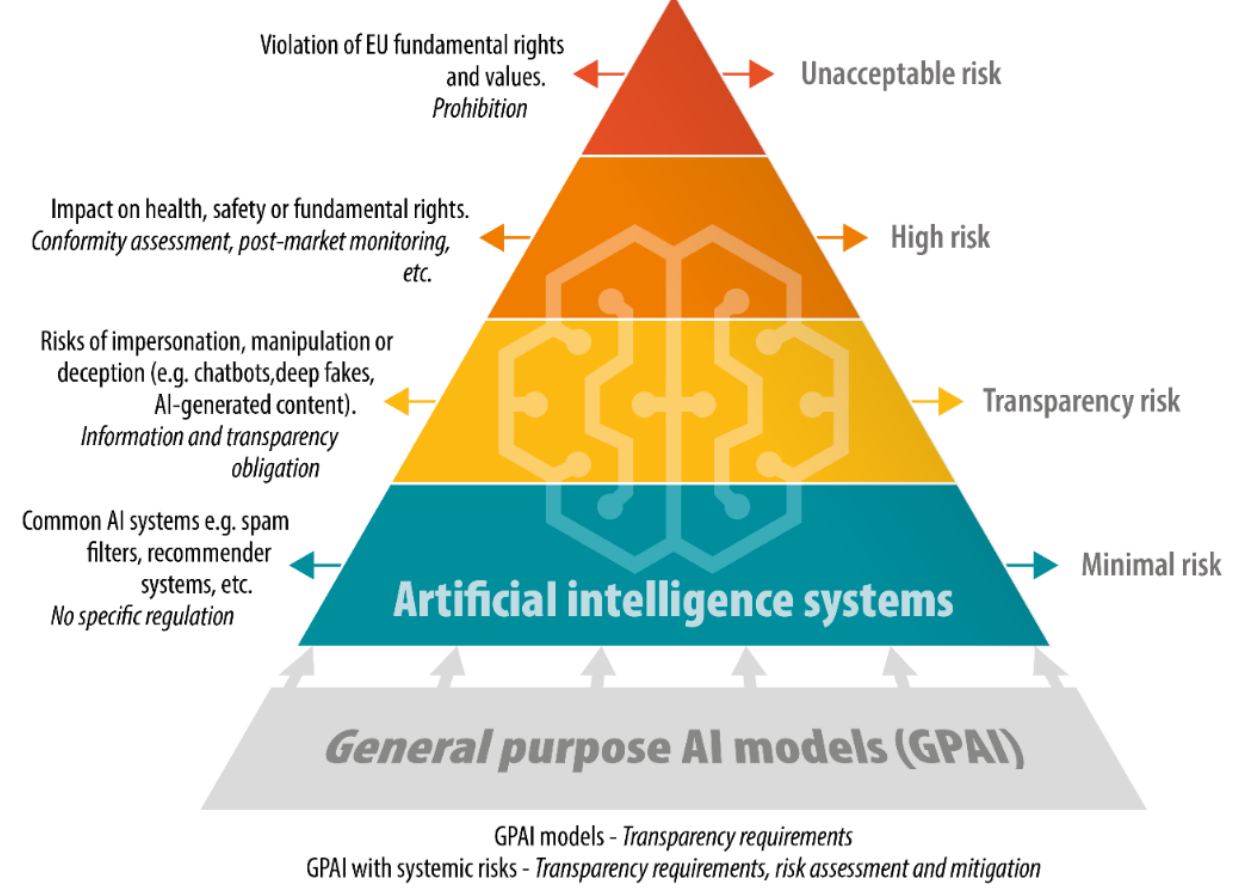
\includegraphics[width=0.75\textwidth]{screen2.png}

\vspace{\baselineskip}
\scriptsize \textbf{Source:} \href{https://www.europarl.europa.eu/RegData/etudes/BRIE/2021/698792/EPRS_BRI(2021)698792_EN.pdf}{AI Act Briefing (EU Parliament)}
\caption{Risk levels defined in the European Union AI Act}
\label{fig:euaiact}
\end{figure}

Systems with \emph{unacceptable risk} are categorically prohibited. These are systems that manipulate human behaviour or that classify people based on their behaviour, socio-economic status, or personal characteristics (''social scoring systems''). Also prohibited is the untargeted scraping of facial images off the internet for purposes of building face recognition databases. Emotion recognition in the workplace or educational institutions is prohibited, except when used for medical or safety reasons. Also prohibited is the use of real-time biometric identification systems in public spaces, such as facial recognition, iris scanners, or others. Biometric categorization to infer race, sexual orientation, political opinions or religious beliefs is also prohibited as posing an unacceptable risk. 

Systems with \emph{high risks} are those that could be expected to pose significant risks to health, safety or the fundamental rights of a person. The EU AI act imposes a registration requirement for AI systems operating in specific sectors that are deemed to present such a high risk. These include: 
\begin{itemize}
  \item Operation of critical infrastructure, for example water or electricity supply, air traffic control,
  \item Education and vocational training,
  \item Employment, worker management and access to self-employment (the latter would capture the so-called ''gig economy'' companies like Uber),
  \item Access to essential private and public services, and benefits,
  \item Law enforcement,
  \item Migration, asylum, and border control,
  \item Assistance in legal interpretation and application of the law.
\end{itemize}

Additionally, AI systems that are incorporated into products governed by EU product safety regulations (toys, cars, medical devices, etc.) are also considered high-risk, but do not have a registration requirement.

For AI systems classified as high-risk, the AI Act imposes several strict regulatory obligations:
\begin{itemize}
  \item \emph{Risk Management and Mitigation}: These systems should include regular risk assessments to identify potential safety risks and risks to fundamental rights. Any risks must be mitigated through appropriate design, testing, and validation processes before the AI system is deployed.

  \item \emph{Data Governance and Quality Requirements}: The data used to train, validate, and test high-risk AI systems must be accurate, relevant, representative, and free from biases that could lead to discriminatory outcomes.

  \item \emph{Logging and Record-Keeping}: To ensure traceability and accountability, developers are required to log the operation of high-risk AI systems, keeping records of system activities, training data, and the decision-making processes of the AI. 

  \item \emph{Transparency and Information Disclosure}: Users of high-risk AI systems must be informed about how the system operates, its intended purpose, and the possible impacts on them. In certain cases, the AI system must provide explanations for its decisions, especially when they affect an individual's rights or freedoms.

  \item \emph{Human Oversight}: The EU AI Act emphasizes the importance of human oversight in the deployment of high-risk AI systems. AI systems should not operate entirely autonomously in critical areas, such as law enforcement or healthcare. Human operators must have the ability to intervene and override AI decisions when necessary to prevent harm or ensure ethical outcomes.
\end{itemize}

Systems that pose a \emph{transparency risk} are those that could be used to impersonate or deceive users or third parties. Typical examples are chat-bots, deep-fake AI systems, and AI generated content. The EU AI act imposes information and transparency obligations on such systems. That is, users must be informed when they are interacting with an AI system, and the output of such systems must be marked and disclosed as AI generated. 

Systems that pose \emph{minimal risk} are the remaining systems that do not fall in the other three categories. There are no regulations for their development or use, nor are there registration requirements. 

Organizations developing or deploying high-risk AI systems will need to undergo compliance assessments, conducted by either the organizations themselves or third-party bodies, depending on the type of AI system involved. Developers will also need to register certain high-risk AI systems in a public EU database, allowing for transparency and public oversight. Non-compliance with the AI Act can lead to significant penalties, including fines. For the most serious infringements, such as deploying prohibited AI systems, the AI Act allows for fines of up to 6\% of a company's global annual turnover. Lesser violations, such as failure to comply with transparency requirements, can result in fines of up to 4\% of global turnover.

In conclusion, the EU AI act is the first legislation that recognizes the risks posed by AI and machine learning systems, and is a first attempt to regulate these systems to reduce or prevent potential harms.


\FloatBarrier

\section{Review Questions}
\paragraph*{Tort Law}
\begin{enumerate}[nosep]
	\item Distinguish between employees and independent contractors. Why is this distinction important in determining vicarious liability?
	\item Discuss the concept of compensatory and punitive damages. How do they differ, and what purpose does each serve in tort law?
	\item In what ways could a business's data collection efforts lead to a claim for intrusion on seclusion? Provide an example.
	\item What is the tort of breach of confidence? How might this tort arise in a business analytics context?
	\item Differentiate between trespass to land and nuisance. How might these torts apply to data collection via drones?
	\item Define negligence and outline the elements required to prove a negligence claim. How does the concept of duty of care apply in a business setting?
	\item Provide an example of how negligence in the development or operation of a predictive model could result in harm or injury.
\end{enumerate}
\paragraph*{Contracts, Licenses, Copyright, and Web Data}
\begin{enumerate}[nosep,resume*]
	\item Define a contract in the context of business analytics. What are some examples of contracts related to data or analytics services?
	\item What is the significance of the Uniform Electronic Commerce Act (UECA) for contracts formed in the digital realm?
	\item Explain the difference between selling data and licensing data in a business analytics context. Provide an example of each.
	\item How can liability and indemnification clauses be used in contracts for predictive models or analytics services?
	\item Define a license and explain the difference between an exclusive, sole, and non-exclusive license.
	\item What is the significance of transferability and sub-licensing in a license agreement?
	\item How does copyright law distinguish between facts and original works? Why is this distinction important for business analytics?
	\item What is the copyright issue related to training predictive models with data? Why is this area still unclear in Canadian law?
	\item What is the Robot Exclusion Protocol (robots.txt)? How does it help limit web crawlers from accessing certain parts of a website?
\end{enumerate}
\paragraph*{PIPEDA}
\begin{enumerate}[nosep,resume*]
	\item What is PIPEDA and what areas of Canadian business does it apply to?
	\item Explain what is meant by ''personal information'' under PIPEDA and provide five examples of personal information.
	\item What types of information are specifically exempt from PIPEDA?
	\item What is the role of the Office of the Privacy Commissioner (OPC) under PIPEDA? What enforcement powers does it hold?
	\item What are the ten Fair Information Principles that form the foundation of PIPEDA?
	\item Discuss the principle of accountability under PIPEDA. What measures must organizations take to comply?
	\item Explain the importance of obtaining valid, informed consent under PIPEDA. What are some examples of situations where explicit consent is required?
	\item Describe some ''no-go zones'' where collecting, using, or disclosing personal information is considered inappropriate, even with consent.
	\item Under what circumstances is opt-out consent considered acceptable by the OPC?
	\item Outline the guidelines provided by the OPC for video data collection. Why is limiting collection important in video surveillance?
	\item Describe the process for disposing of personal information under PIPEDA. What are the differences between clearing, purging, and destroying information?
	\item What steps must organizations take to ensure the accuracy of personal information under PIPEDA?
	\item What safeguards does PIPEDA require organizations to implement to protect personal information?
	\item What is "employee snooping," and what steps can organizations take to prevent it?
	\item What rights do individuals have under PIPEDA regarding access to their personal information held by an organization?
	\item Explain how organizations must respond to requests for correction or amendment of personal information under PIPEDA.
	\item What does PIPEDA require with respect to mandatory breach reporting? In what circumstances must organizations report a breach to the OPC?
	\item Describe the role of contractual agreements in ensuring PIPEDA compliance when personal information is shared with third parties.
	\item How must organizations handle information that is accidentally collected or received under PIPEDA?
\end{enumerate}
\paragraph*{Bill C-27, AIDA, and the EU AI Act}
\begin{enumerate}[nosep,resume*]
	\item What is the main purpose of the proposed Artificial Intelligence and Data Act (AIDA)?
	\item What is the significance of ''high-impact AI systems'' under AIDA? Provide two examples of such systems.
	\item Explain what is meant by ''biased output'' under AIDA and give an example of how this could occur in an AI system.
	\item What six principles guide the requirements under AIDA for organizations using high-impact AI systems?
	\item Discuss the principle of human oversight and monitoring. Why is it important in the context of high-impact AI systems?
	\item Explain the principle of transparency under AIDA. What kind of information should organizations provide about high-impact AI systems?
	\item Describe the safety principle in AIDA. How should organizations approach potential harms from AI systems?
	\item Define the validity and robustness principle. Why is it critical to ensure AI systems operate reliably?

	\item What activities with respect to high-impact AI systems are regulated under AIDA?
	\item What are the responsibilities of organizations when making a high-impact AI system available for use?

	\item Discuss the enforcement powers of the Minister of Industry, Science, and Economic Development under AIDA.
	\item What are the three new criminal offences introduced by AIDA? Provide an example for each.

	\item What are some examples of AI systems categorized as posing unacceptable risk under the European Union AI Act?
	\item How does the European Union AI Act handle AI systems that pose transparency risks, such as chatbots and deep-fakes?
	\item Compare the regulation of high-risk AI systems in AIDA and the European Union AI Act. What are the similarities and differences?
\end{enumerate}

